\begin{evenBlock}{3+Help vs. 4}

\begin{minipage}[t]{\linewidth}
    \centering
    
    \begin{minipage}{.3\linewidth} % Left column and width
        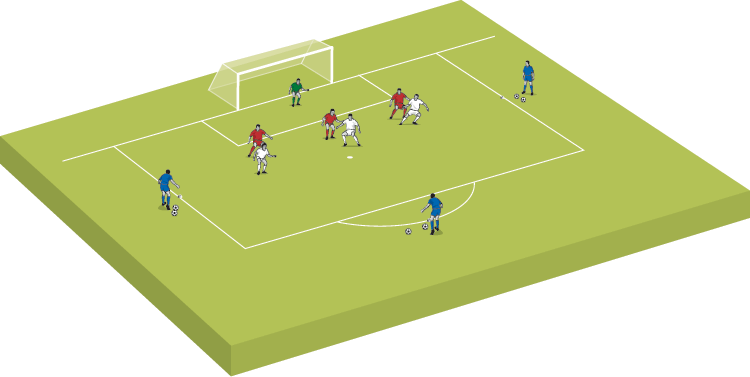
\includegraphics[width=\textwidth]{../img/Trimmed/SecureTheBox1}
    \end{minipage}
    \hspace{0.05\linewidth}
    \begin{minipage}{.6\linewidth} % Left column and width
        \textbf{Drill Description:}
        This drill is ideally played with 10 players, 4 defensive players + 1 keeper and 5 attacking players.  Thsi uses one half the field, the 3 Attacking players start that the mid field line.  Two mid fielders are on the defensive side of the midfield line.  The mid fielders can't cross the line, they can be passed to and then pass back to one of the three forwards or the other mid fielder.  The striker starts the drill by passing to one of his wings.  The 4 defensive backs guard the box and once the ball is passed can move to defend.  Defense wins if the ball is cleared.  Offense wins if they score or win a corner kick.
        
        \textbf{Coaching Points:}
        \begin{itemize}
            \setlength{\itemsep}{0pt}
            \setlength{\parskip}{0pt}
            \setlength{\parsep}{0pt}
            \item Remind the defense about the funnel positioning.
            \item Explain how to mark a player goal side (defender between the attacker and goal).
            \item Explain how to mark a player ball side (defender between the attacker and the ball).
            \item Explain how to mark a player both goal side and ball side - defender marks the attacker goal side but is a few feet (steps) closer to the ball than the attacker.
            \item Defenders should communicate if they want to defend a zone or a man.  Explain to them how this can work.
            \item Attackers look for open space.
            \item Mid fielders look for open space on the opposite side of the field.
        \end{itemize}

    \end{minipage}
\end{minipage}

\end{evenBlock}